% !TEX TS-program = pdflatex
% !TEX encoding = UTF-8 Unicode

% This is a simple template for a LaTeX document using the "article" class.
% See "book", "report", "letter" for other types of document.

\documentclass[11pt, titlepage]{article} % use larger type; default would be 10pt

\usepackage[utf8]{inputenc} % set input encoding (not needed with XeLaTeX)

%%% Examples of Article customizations
% These packages are optional, depending whether you want the features they provide.
% See the LaTeX Companion or other references for full information.

%%% PAGE DIMENSIONS
\usepackage{geometry} % to change the page dimensions
\geometry{a4paper} % or letterpaper (US) or a5paper or....
\geometry{margin=2cm, headsep=5mm, includefoot, includehead}

\usepackage{graphicx} % support the \includegraphics command and options

% \usepackage[parfill]{parskip} % Activate to begin paragraphs with an empty line rather than an indent

%%% PACKAGES
\usepackage{booktabs} % for much better looking tables
\usepackage{array} % for better arrays (eg matrices) in maths
\usepackage{paralist} % very flexible & customisable lists (eg. enumerate/itemize, etc.)
\usepackage{verbatim} % adds environment for commenting out blocks of text & for better verbatim
\usepackage{subfig} % make it possible to include more than one captioned figure/table in a single float
% These packages are all incorporated in the memoir class to one degree or another...

%%% HEADERS & FOOTERS
\usepackage{fancyhdr} % This should be set AFTER setting up the page geometry
\pagestyle{fancy} % options: empty , plain , fancy
\fancyhead{}
%%% SECTION TITLE APPEARANCE
\usepackage{sectsty}
\allsectionsfont{\sffamily\mdseries\upshape} % (See the fntguide.pdf for font help)
% (This matches ConTeXt defaults)

%%% ToC (table of contents) APPEARANCE
\usepackage[nottoc,notlof,notlot]{tocbibind} % Put the bibliography in the ToC
\usepackage[titles,subfigure]{tocloft} % Alter the style of the Table of Contents
\renewcommand{\cftsecfont}{\rmfamily\mdseries\upshape}
\renewcommand{\cftsecpagefont}{\rmfamily\mdseries\upshape} % No bold!

\usepackage{lastpage}
\usepackage{rotating}
%---------- Enable IEEEtran.bst configurations ------
\usepackage{IEEEtrantools}
%----------------------------------------------------

%%% END Article customizations

%%% The "real" document content comes below...

%%% Header %%%%%%%%%%%%%%%%%%%%%%%%%%%%%
\setlength{\headheight}{52.4842pt}
\lhead{EH2760 Management of Projects \\
       Assignment 1 \\
       ESS-CAR/ESS-NW \\
       Leon Fernandez, leonfe@kth.se}
\rhead{Project Plan \\
       \today \\
       Version 1 \\
       \thepage(\pageref{LastPage})}
\renewcommand{\headrulewidth}{0.4pt}
%%%%%%%%%%%%%%%%%%%%%%%%%%%%%%%%%%%%%%%%

%%% Footer %%%%%%%%%%%%%%%%%%%%%%%%%%%%%
%\cfoot{blablablabla}
%\renewcommand{\footrulewidth}{0.4pt}
%%%%%%%%%%%%%%%%%%%%%%%%%%%%%%%%%%%%%%%%

%\title{ESS-CAR/ESS-NW Project Plan}
%\author{Jonas Ekman \\
%        Leon Fernandez \\
%        Yini Gao \\
%        Fredrik Hyyrynen \\
%        Jacob Kimblad \\
%        Yifan Ruan
%        }
%\date{} % Activate to display a given date or no date (if empty),
         % otherwise the current date is printed 

\begin{document}
%\maketitle
\bstctlcite{BSTcontrol} % IEEEtran.bst controls enabled


%----------------------------------------------------------------------------------------
%	TITLE PAGE
%----------------------------------------------------------------------------------------

\begin{titlepage} % Suppresses displaying the page number on the title page and the subsequent page counts as page 1
	\newcommand{\HRule}{\rule{\linewidth}{0.5mm}} % Defines a new command for horizontal lines, change thickness here
	
	\center % Centre everything on the page
	
	%------------------------------------------------
	%	Headings
	%------------------------------------------------
	
	\textsc{\LARGE EH2760 Management of Projects}\\[1.5cm] % Main heading such as the name of your university/college
	
	\textsc{\Large ESS-CAR/ESS-NW}\\[0.5cm] % Major heading such as course name
	
	\textsc{\large Stockholm, Sweden}\\[0.5cm] % Minor heading such as course title
	
	%------------------------------------------------
	%	Title
	%------------------------------------------------
	
	\HRule\\[0.4cm]
	
	{\huge\bfseries Project Plan}\\[0.4cm] % Title of your document
	
	\HRule\\[1.5cm]
	
	%------------------------------------------------
	%	Author(s)
	%------------------------------------------------
	
	\begin{minipage}{0.4\textwidth}
		\begin{flushleft}
			\large
                        \textsc{Jonas Ekman}
			\\
			\textsc{Yini Gao}
                        \\
                        \textsc{Jacob Kimblad}
		\end{flushleft}
	\end{minipage}
	~
	\begin{minipage}{0.4\textwidth}
		\begin{flushright}
			\large
                        \textsc{Leon Fernandez}
			\\
			\textsc{Fredrik Hyyrynen}
                        \\
                        \textsc{Yifan Ruan}
		\end{flushright}
	\end{minipage}
	
	% If you don't want a supervisor, uncomment the two lines below
        % and comment the code above
	%{\large\textit{Author}}\\
	%John \textsc{Smith} % Your name
	
	%------------------------------------------------
	%	Date
	%------------------------------------------------
	
	\vfill\vfill\vfill % Position the date 3/4 down the remaining page
	
	{\large\today} % Date, change the \today to a set date if you want
                       % to be precise
	
	%------------------------------------------------
	%	Logo
	%------------------------------------------------
	
	%\vfill\vfill
	%
\includegraphics[width=0.2\textwidth]{placeholder.jpg}\\[1cm]
        % Include a department/university logo
        % - this will require the graphicx package
	 
	%-------------------------------------------------------------------
	
	\vfill % Push the date up 1/4 of the remaining page
	
\end{titlepage}

%-------------------------------------------------------------------------


\section*{Background}
Advanced Driver Assistance Systems (ADAS) is one of the hottest research
areas in the automotive industry. ADAS should be capable of sensing the
vehicle's surroundings, as well as vehicle's own status. To achieve those
abilities, multiple sensors and Embedded Control Units (ECUs) are used
in the ADAS and a network inside the vehicle is established to combine
the data gathered from different nodes.

The two projects ''ESS-Car Embedded Services for a Self-Adaptive Car'' and
''ESS-Network Embedded services for Self-Adaptive Networking'' were
provided by professor De-Jiu Chen at KTH Royal Institute of Technology.
The idea of our projects are from Viktor Karlquist's Master's thesis
\cite{viktor}. He presented a design and implementation of an automotive
experimental platform for ADAS, and the ''ESS-Car'' team from last year's
MF2063 course round has already built a autonomous vehicle prototype based
on the thesis \cite{old_ess}. Our projects will be focused on the
development and extension of the prototype. Instead of traditional IP
networks, software defined networking, which centralizes the control
plane in the network and allows for a better granular and agile network
management, will be implemented by ''ESS-NW'' team. ''ESS-Car'' team will
implement error injectors on the new prototype which makes the car more
autonomous.

\subsection*{Reference Documents}
\begin{itemize}
    \item EH2760 course-pm \cite{eh2760_pm}
    \item ESS-CAR and ESS-NW entries in the MF2063 project catalog
        \cite{projects}
\end{itemize}

\section{Goals}
The goals of the project can be divided into two parts, goals concerning
the network implementation on the car and goals concerning the remaining
software and hardware system architecture of the car. As both parts are
heavily tied into each other some of the sub-goals are dependent on
sub-goals from the opposing . The overarching goal of the network
implementation is of a more exploratory nature as it is a problem that has
not been studied clearly, thus the project aims to explore what different
network implementations can be beneficial in this type of infrastructure.
The overarching goal can be stated as ''The goal of the project is to
reconfigure the network using SDN-switches and a Raspberry Pi as a SDN
controller''. The overarching goal for the software and hardware system
architecture can be stated as ''The goal of the project is to increase the
robustness by revising the existing architecture and implementing
additional features such as vision control and a display service.''  Not
related to the technical aspects of the car, but rather the ambitions of
the project members, are also the business goals of the project.

\subsection{Technical Goals}
The technical subgoals are divided up into two parts. Subgoals concerning
the ethernet network which takes care of all of the communication between
different parts of the system. Subgoals concerning the hardware and system
architecture which implements all of the functionalities of the system
except for the network communication.


\subsubsection{Hardware and Software System Architecture}
As discussed in the background, the project builds on an existing
architecture. Thus most goals consists of improving the existing
architecture or examining alternative implementations. The first subgoal
consists of making the system more robust by extending the hardware
architecture. This should be done such that there is one unique
microprocessor for each sensor and actuator in the system while maintaining
the existing functionalities of the car. The next subgoal is to monitor the
operations of the ECU’s such that the car can be made fail-safe by
implementing fault-detection, watchdogs and battery level indication.
The next subgoal is to develop a formal boot- and shutdown-sequence such
the the car becomes reliable and fail-safe under normal operation. The
final subgoal is to extend the functionality of the existing system by
setting up a camera module and choosing an AI algorithm to detect some
external stimuli such as a traffic sign such that the rest of the system
can react to it (choosing the appropriate speed or steering for example). 
\begin{figure}
    \centering
    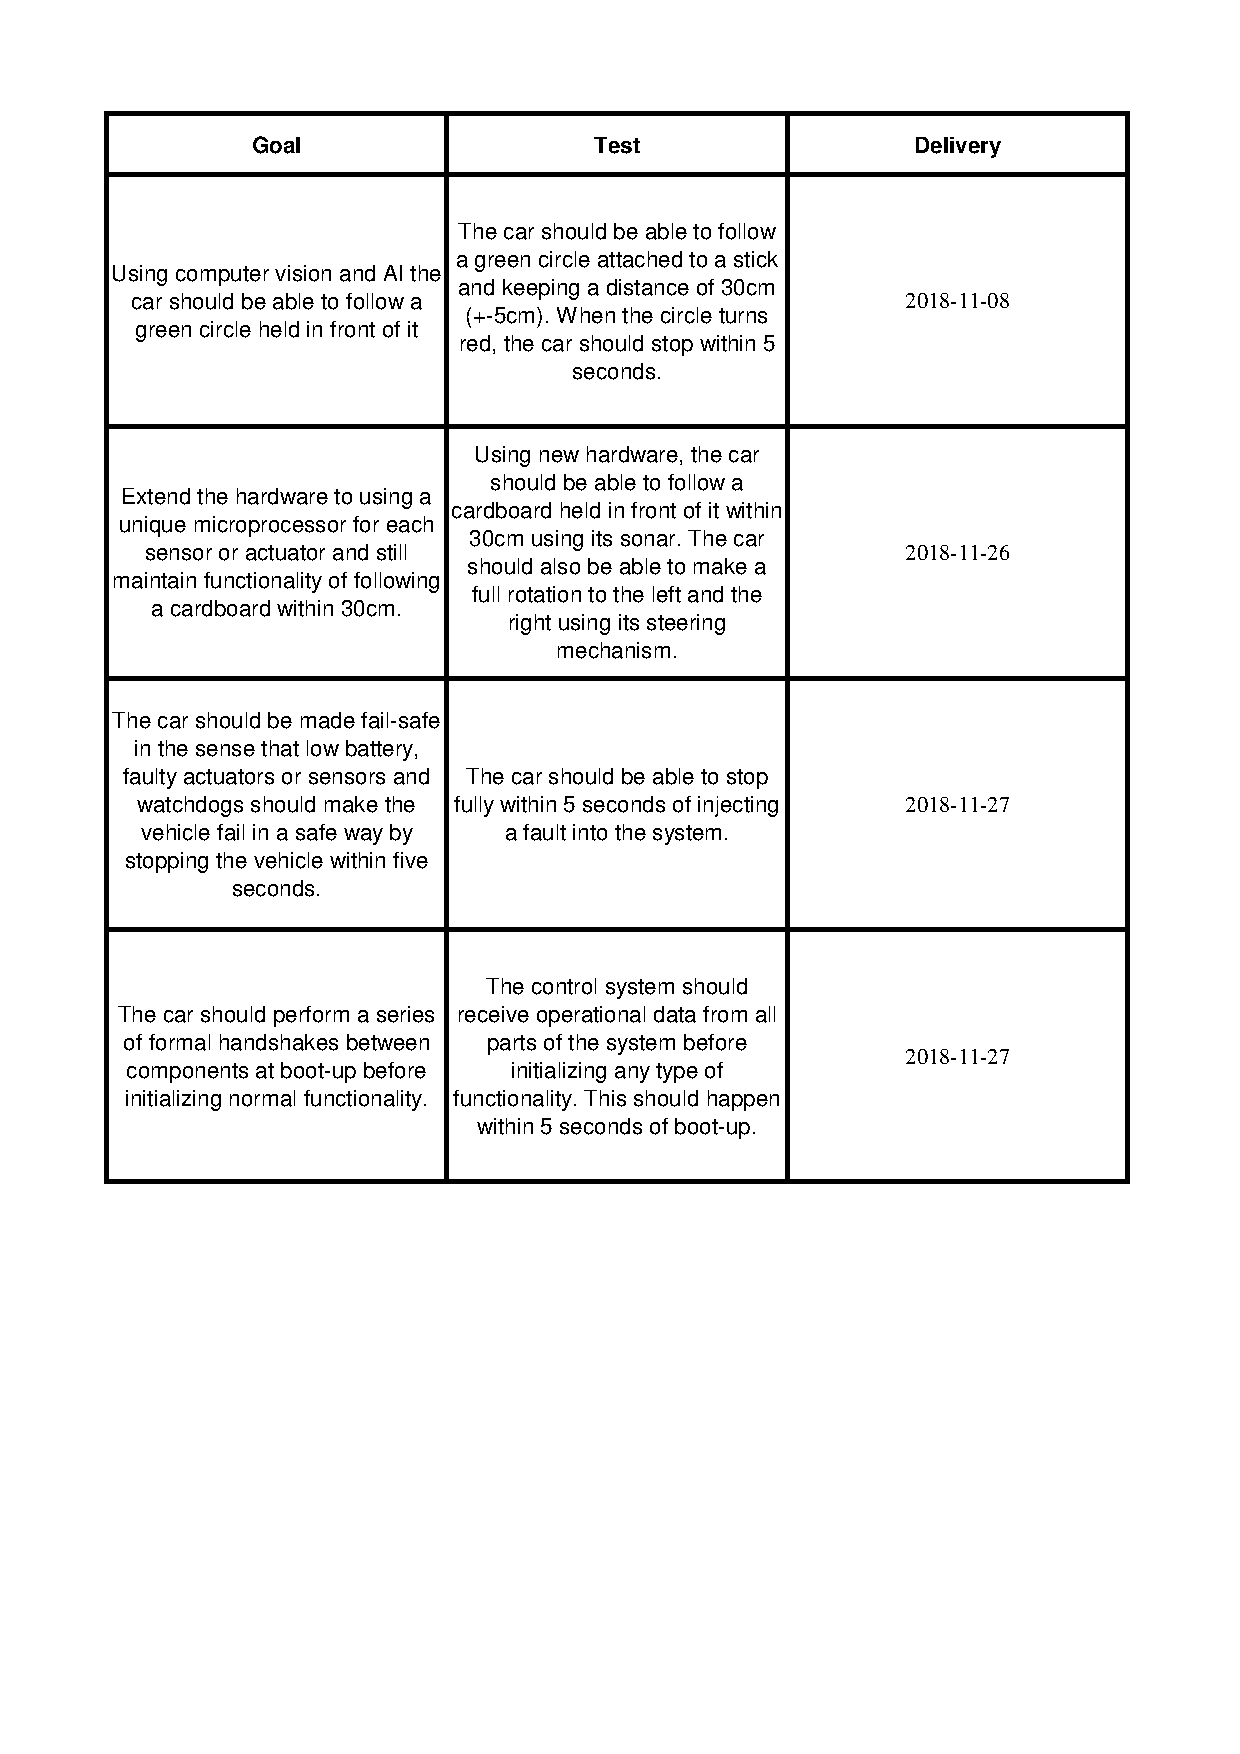
\includegraphics[scale=0.6]{goals_arch.pdf}
    \caption{The goals and associated tests for the system architecture.}
    \label{fig:goals_arch}
\end{figure}

\subsubsection{Network Goals}
The first subgoal is to assemble the car and set up the physical layer
which includes the SDN-switches and the hardware running the SDN-controller
(connecting everything using ethernet cables and powering it up).
Another goal is that the SDN-controller needs to be picked from given
specifications such that it can run on a Raspberry Pi which is part of
the system, and that it can contact the specific SDN-switches that has
already been chosen. When choosing the SDN-controller it should also be 
put into consideration that it can have an impact whether or not the
remaining two goals can be met. The remaining two goals consists of
customizing the SDN-network in different ways. The first one is to
explore how the SDN-controller can be used to manually assign different
pre-configured routes in the network such that packets that are sent from
any given node to any other given node are guaranteed to take a
specifically assigned route through the network. The last goal is to
extend this functionality by automatically reassigning routes in the
network based on given a set of given rules and circumstances in the
network. This means, for example, that if we detect congestion in some
part of the network we can take action to either reroute some packages
or simply drop them depending on their criticality.
\begin{figure}
    \centering
    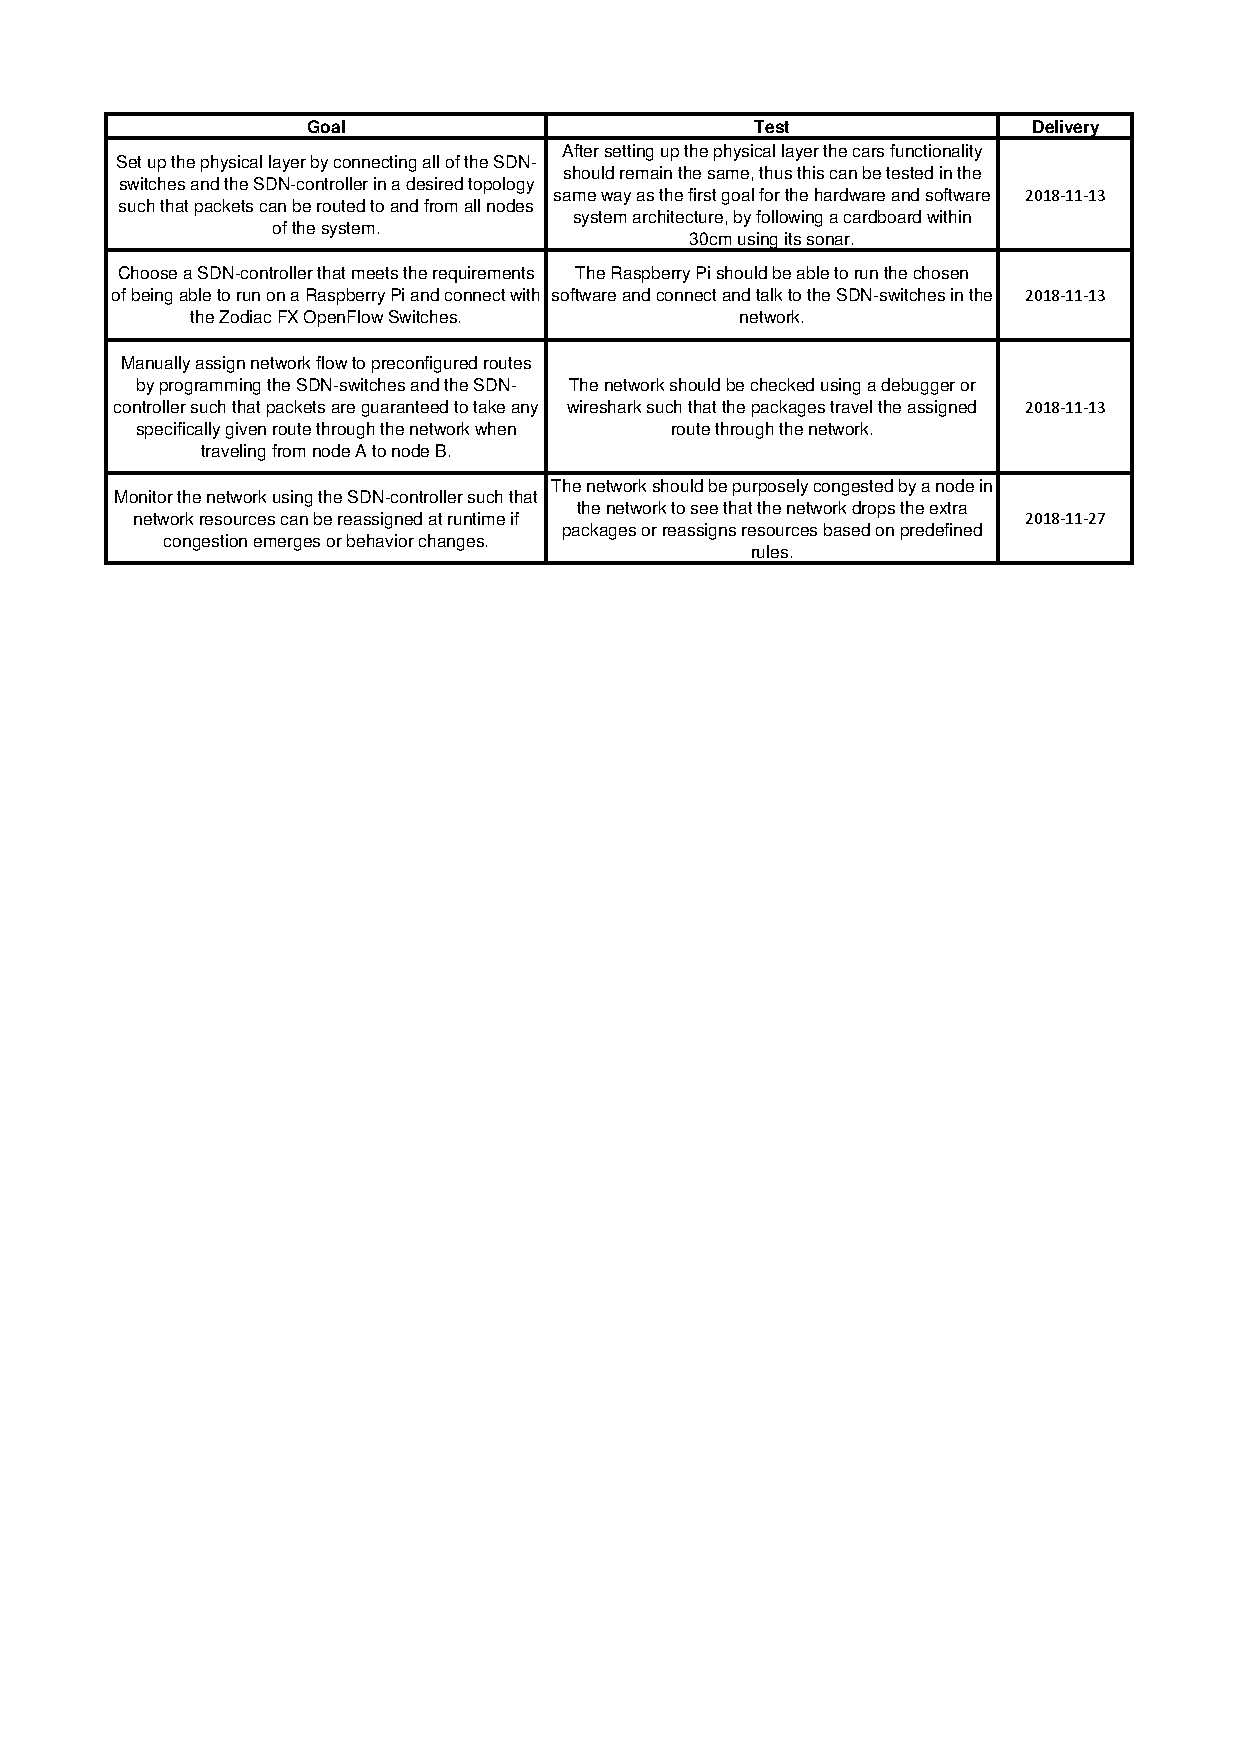
\includegraphics[scale=0.6]{goals_nw.pdf}
    \caption{The goals and associated tests for the network.}
    \label{fig:goals_nw}
\end{figure}

\subsection{Business Goals}
The first subgoal is to assemble the car and set up the physical layer,
which includes the SDN-switches and the SDN-controller. This is a
dependency the other goals. 
\begin{figure}
    \centering
    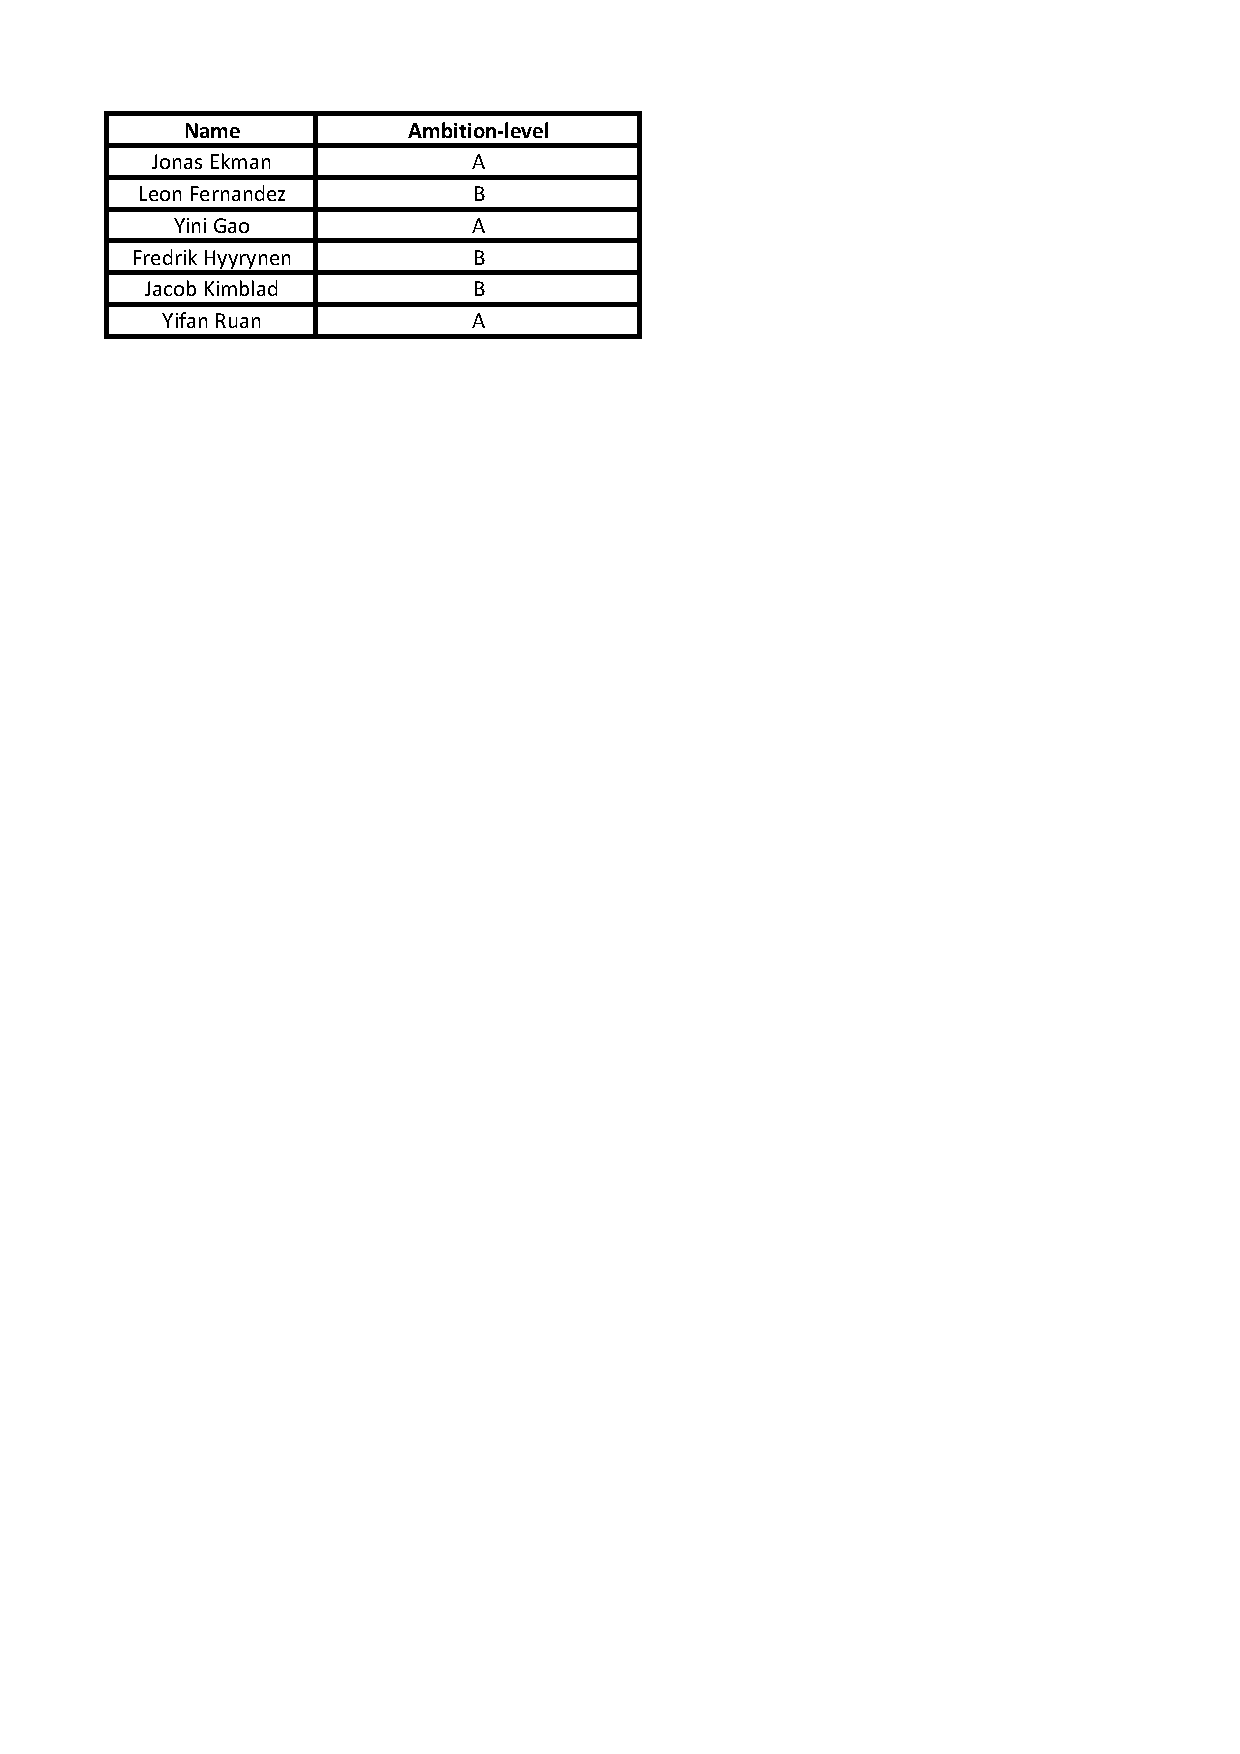
\includegraphics[scale=0.6]{goals_bs.pdf}
    \caption{Non-technical goals for the projects.}
    \label{fig:goals_bs}
\end{figure}
\section{Organization}
The requirements of the project were divided into a number of topics,
with each team member being focused on two topics. Additionally, Leon and
Fredrik have been appointed roles of Project Manager and Secretary,
respectively.

\subsection{People}

\subsubsection{Project Members}
\begin{itemize}
\item Fredrik Hyyrynen, fhyy@kth.se, Software and Computer Vision, Secretary
\item Jacob Kimblad, jacobki@kth.se, Software and Control
\item Jonas Ekman, jonekm@kth.se, Network and Electronics
\item Leon Fernandez, leonfe@kth.se, Network and Software, Project Manager
\item Yifan Ruan, yifanr@kth.se, Control and Electronics
\item Yini Gao, yini@kth.se, Computer Vision and Software
\end{itemize}

\subsubsection{Stakeholders}
\begin{itemize}
    \item Dejiu Chen, chen@md.kth.se, Stakeholder, Supervisor
    \item Matthias Becker, mabecker@kth.se, Stakeholder, Supervisor
\end{itemize}


\subsection{Topics and Roles Elaboration}
\begin{itemize}
\item[Software] - Consists of scheduling the tasks running at the different
    nodes in the system, managing the bootstrapping of the system upon
    startup and lastly, writing code for the arduino nodes
\item[Computer Vision] - Consists of setting up the Raspberry Pi + Camera
    subsystem and implementing the commputer vision algorithm
\item[Control] - Consists of devising and implementing the main
    control algorithm that will run on one of the nodes
\item[Network] - Consists of configuring the SDN switches and SDN controller
    as well as writing the application-layer programs that the nodes
    use to communicate
\item[Electronics] - Consists of doing the PCB design for the
    ''motherboard'' in the car as well as mounting the sensors and 
    wiring in the car
\item[Project Manager] - Consists of communicating with stakeholders, 
    schedule and lead meetings and handling parts orders
\item[Secretary] - Consists of taking notes during meetings and
    being a temporary managar in the absence of the project manager
\end{itemize}

\section{Project Model}
Figure \ref{fig:project_model} and \ref{fig:project_model2} shows the
model for the project. The most important milestones are also present in
\ref{fig:goals_arch} and \ref{fig:goals_nw}.

\begin{figure}
    \centering
    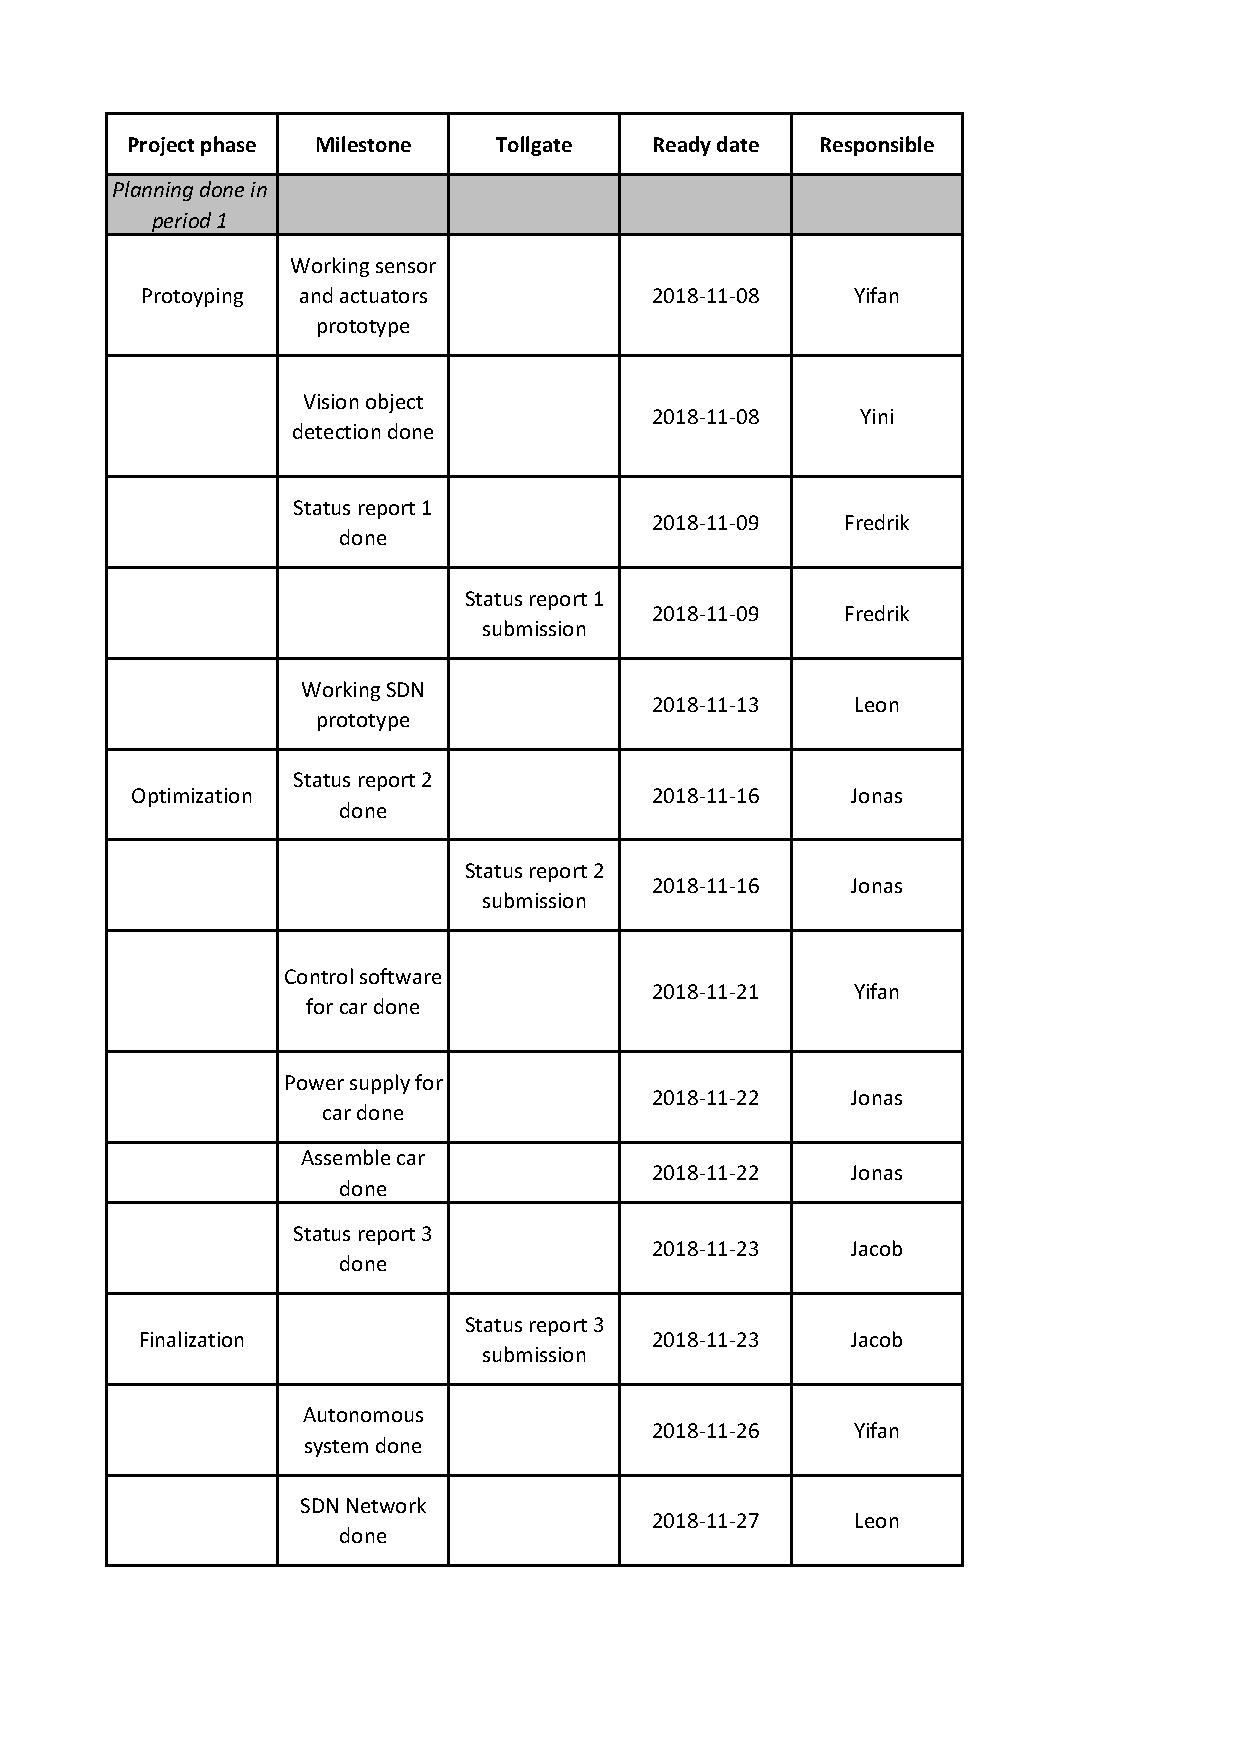
\includegraphics[scale=0.7]{project_model.pdf}
    \caption{The project model.}
    \label{fig:project_model}
\end{figure}
\begin{figure}
    \centering
    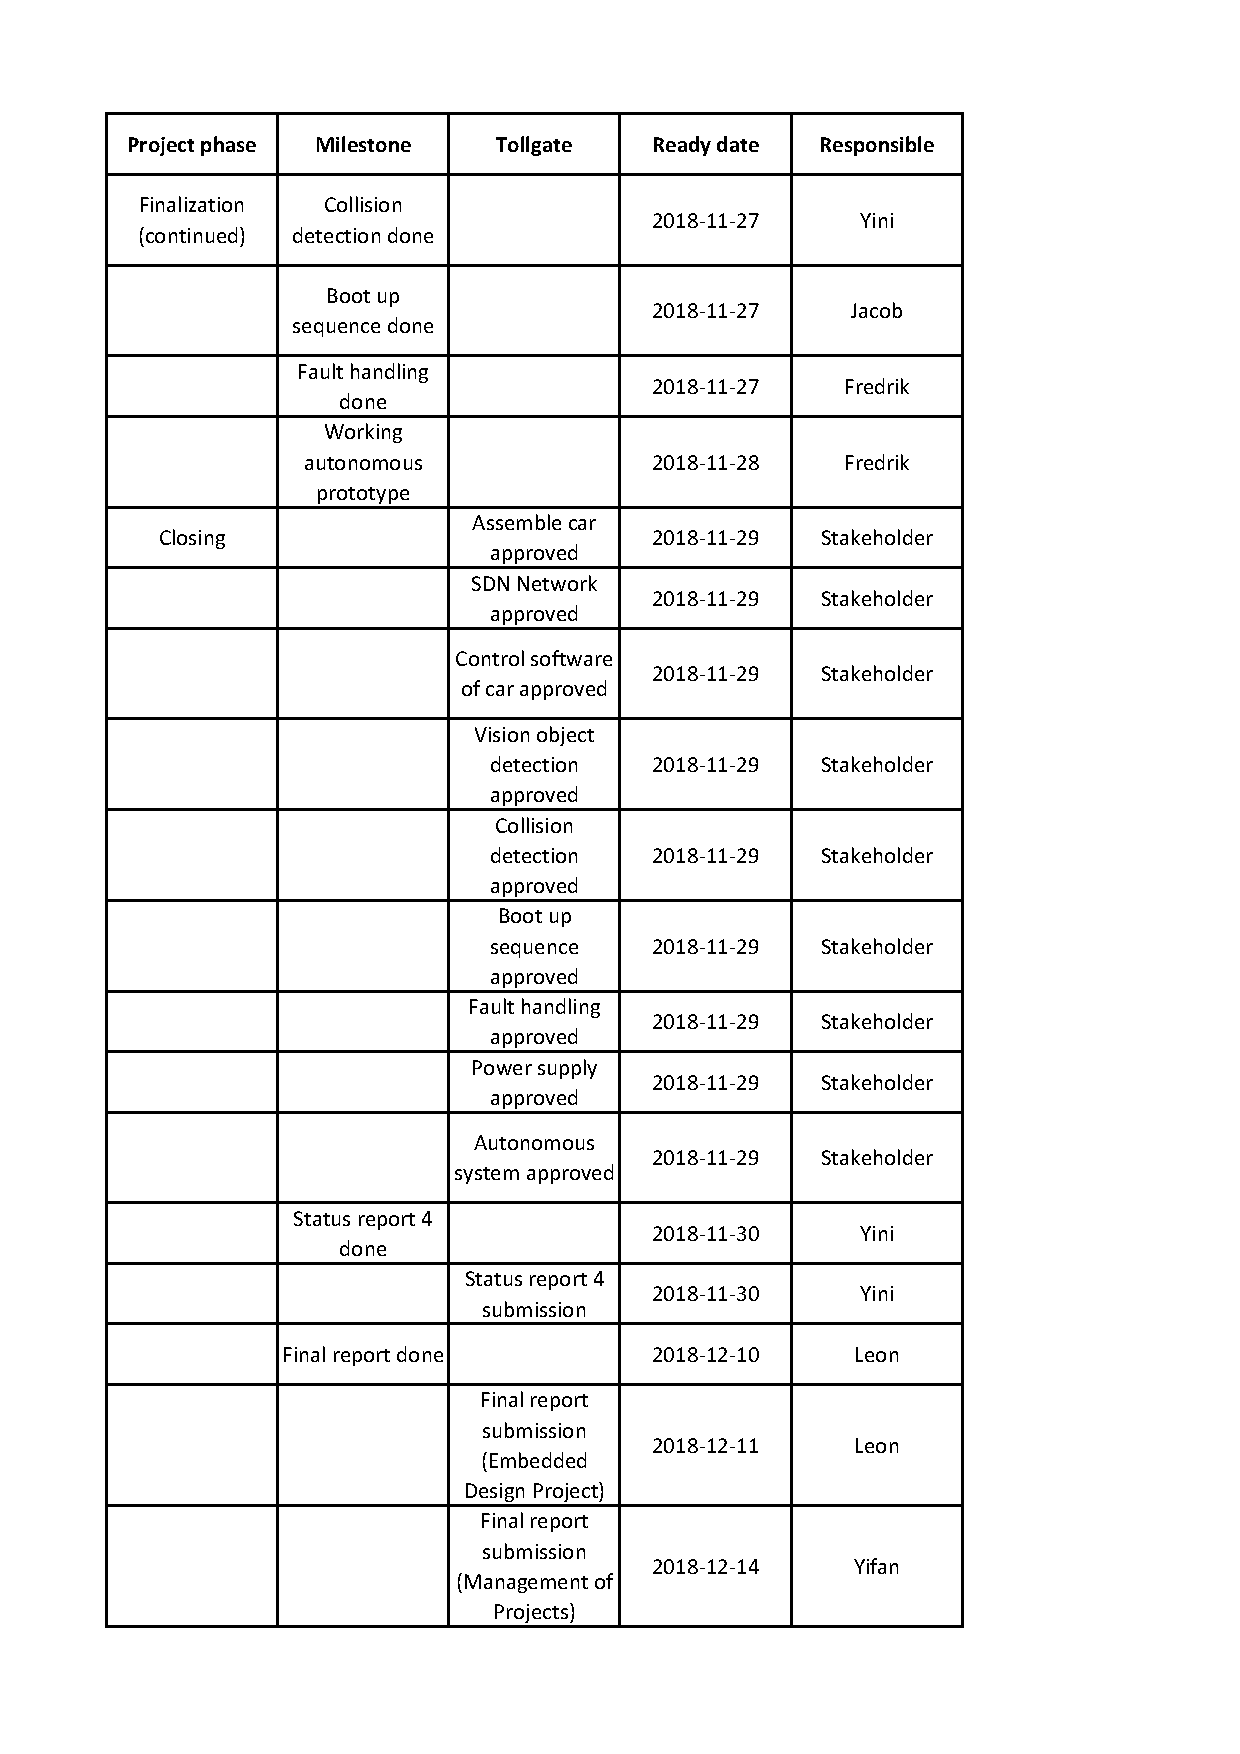
\includegraphics[scale=0.7]{project_model2.pdf}
    \caption{The project model, part 2.}
    \label{fig:project_model2}
\end{figure}




\section{Commentary: Time Plan}
The timeplan has been derived from the WBS and deadlines in EH2760 and MF2063. The timeplan is subject to change
depending on if milestones are completed on their deadlines or not. Tollgates have been intentionally placed on Thursday's
since the stakeholder meetings will take place on those days and thus, the progress can be evaluated.

\section{Commentary: Resource Plan}
The resource plan was based on the number of man-hours available. This was in turn based on the number of credits (hp) that
the course consists of in period 2, which is 6 hp per person. The total number of man-hours available is 960.

\section{Risk Analysis}
\begin{figure}
    \centering
    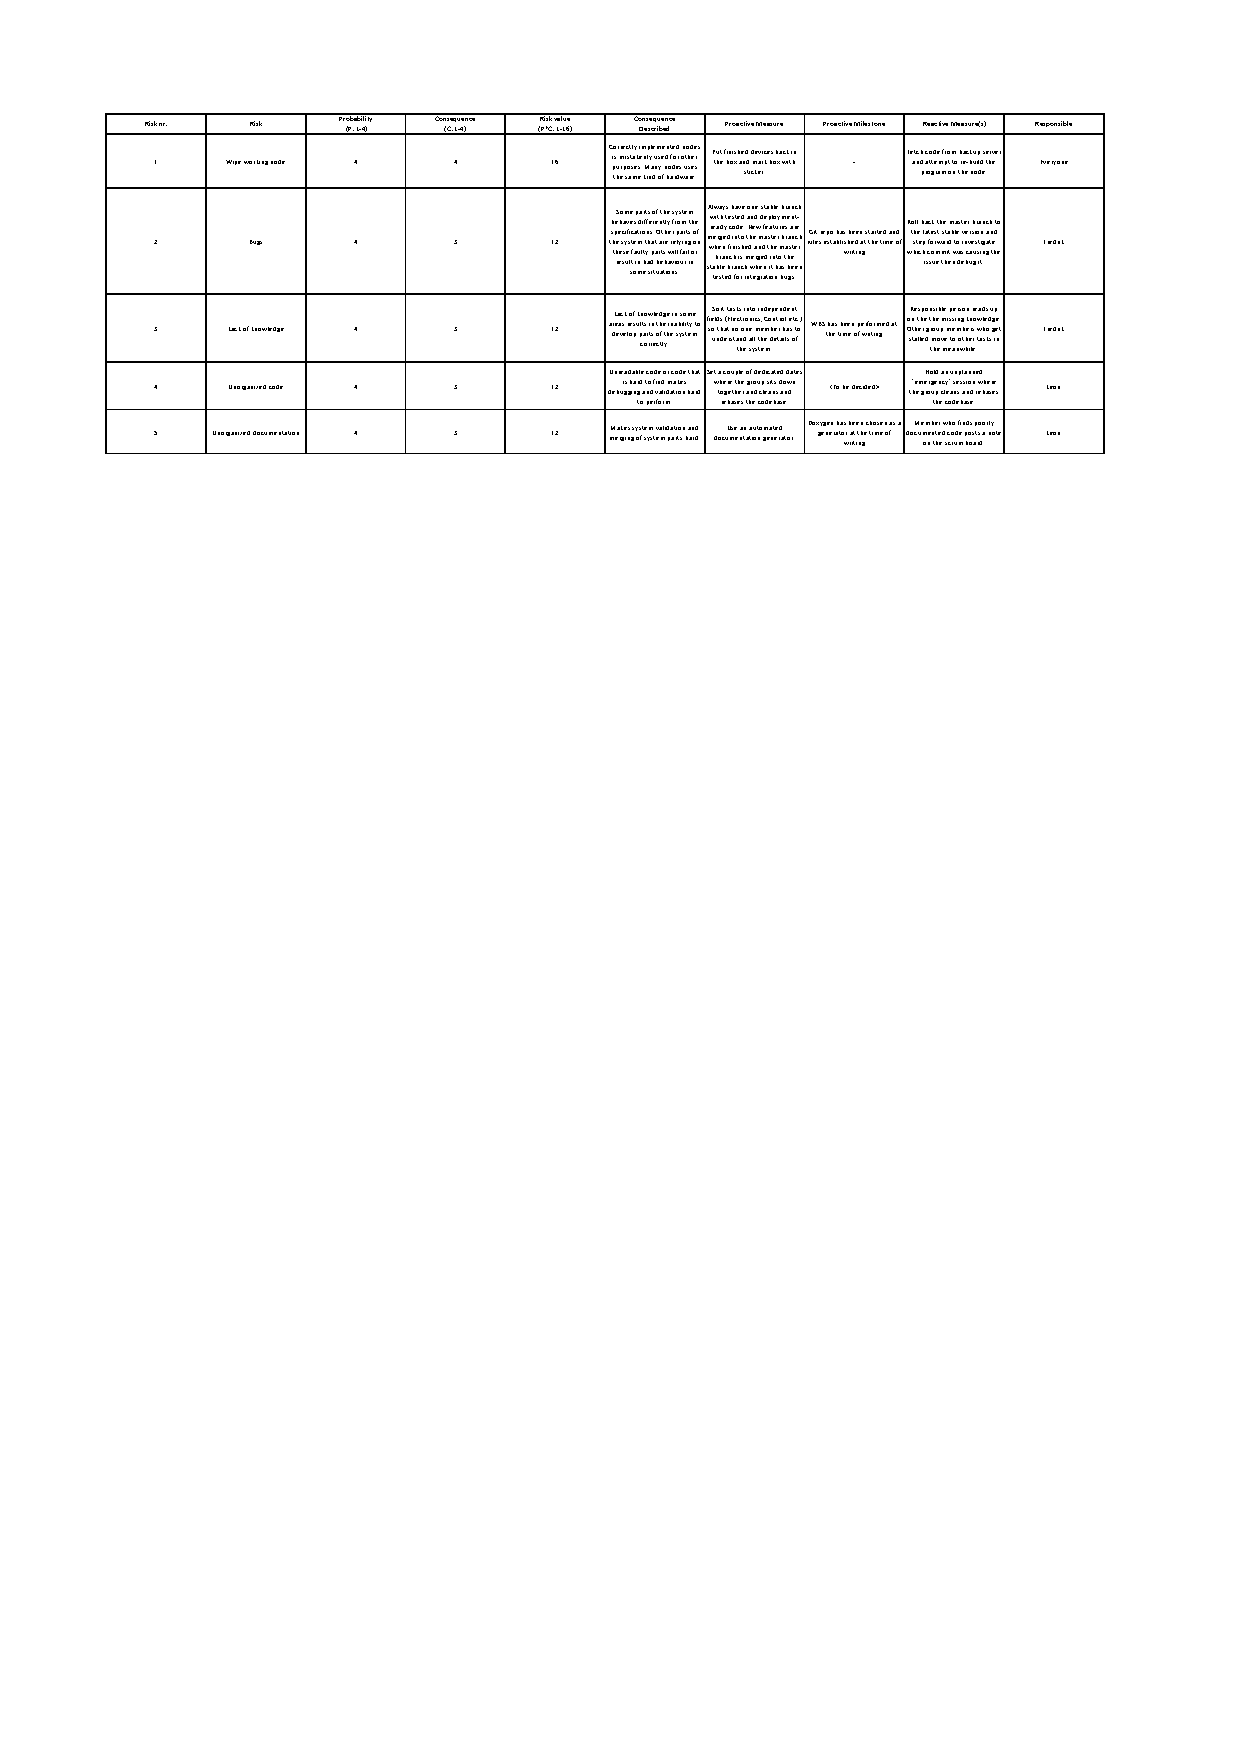
\includegraphics{risks.pdf}
    \caption{A risk matrix for the top five risks.}
    \label{fig:risks}
\end{figure}

\section{Communication}
The main communications channel used is the kth e-mail. Meetings and
scheduling is handled with Microsoft Outlook. For shorter and less
important messages, Slack is used. Slack also interfaces with 
Trello, Google Drive and Github, which facilitates keeping the
documentation up to date. Physical meetings takes place on a
weekly basis during which progress and possible issuesand possible issues are discussed.

\section{Documentation}
Documentation is a critical part during software development project. It is
a good way to communicate the implementation of everyone's work. So, we
need to keep documentation concise and interpretable, for example, overviews
and roadmaps can be shown in our documentation to let other teammates
know about the work in a short time. Only important information like what is
the underlying communication architecture and what type of data it outputs
should be elaborate in documentation. Another significant point is the
accuracy of the documentation due to some future work will be done base on
it. Indexing and linking should also be added to our documentations as
references project.
We use Google Drive and GitHub to manage our documentations since
Google Drive allows us to work on the documentation simultaneously and
GitHub provides control of builds in case of mis-deleting. Another reason we
choose to upload our document to the cloud is that typically the well-known
cloud drive will have good maintenance work. In this case, we normally won’t
lose any important document if we store them on the server.
In our project, documentation will be created throughout the entire project
development lifecycle. And we should write our documents in a iterate way,
which means that we should update our documents after getting some
feedback during the whole development process. For instance, we are
keeping changing the description of a programming code when we add new
parts of it or if someone in the group gives feedback in case of not
readable documents. Finally, we should treat our documentation like
requirements. We need to estimate the priority of our documents and deal
with the most important one first. This priority may change during the
development process and some of documents can even be removed, which
is fully depends on the project's demand.

\clearpage
\bibliography{ESS-CARNW_2018_projectplan_1}
\bibliographystyle{IEEEtran}

\clearpage
\appendix
\section{Time Plan}
\begin{sidewaysfigure}
    \centering
    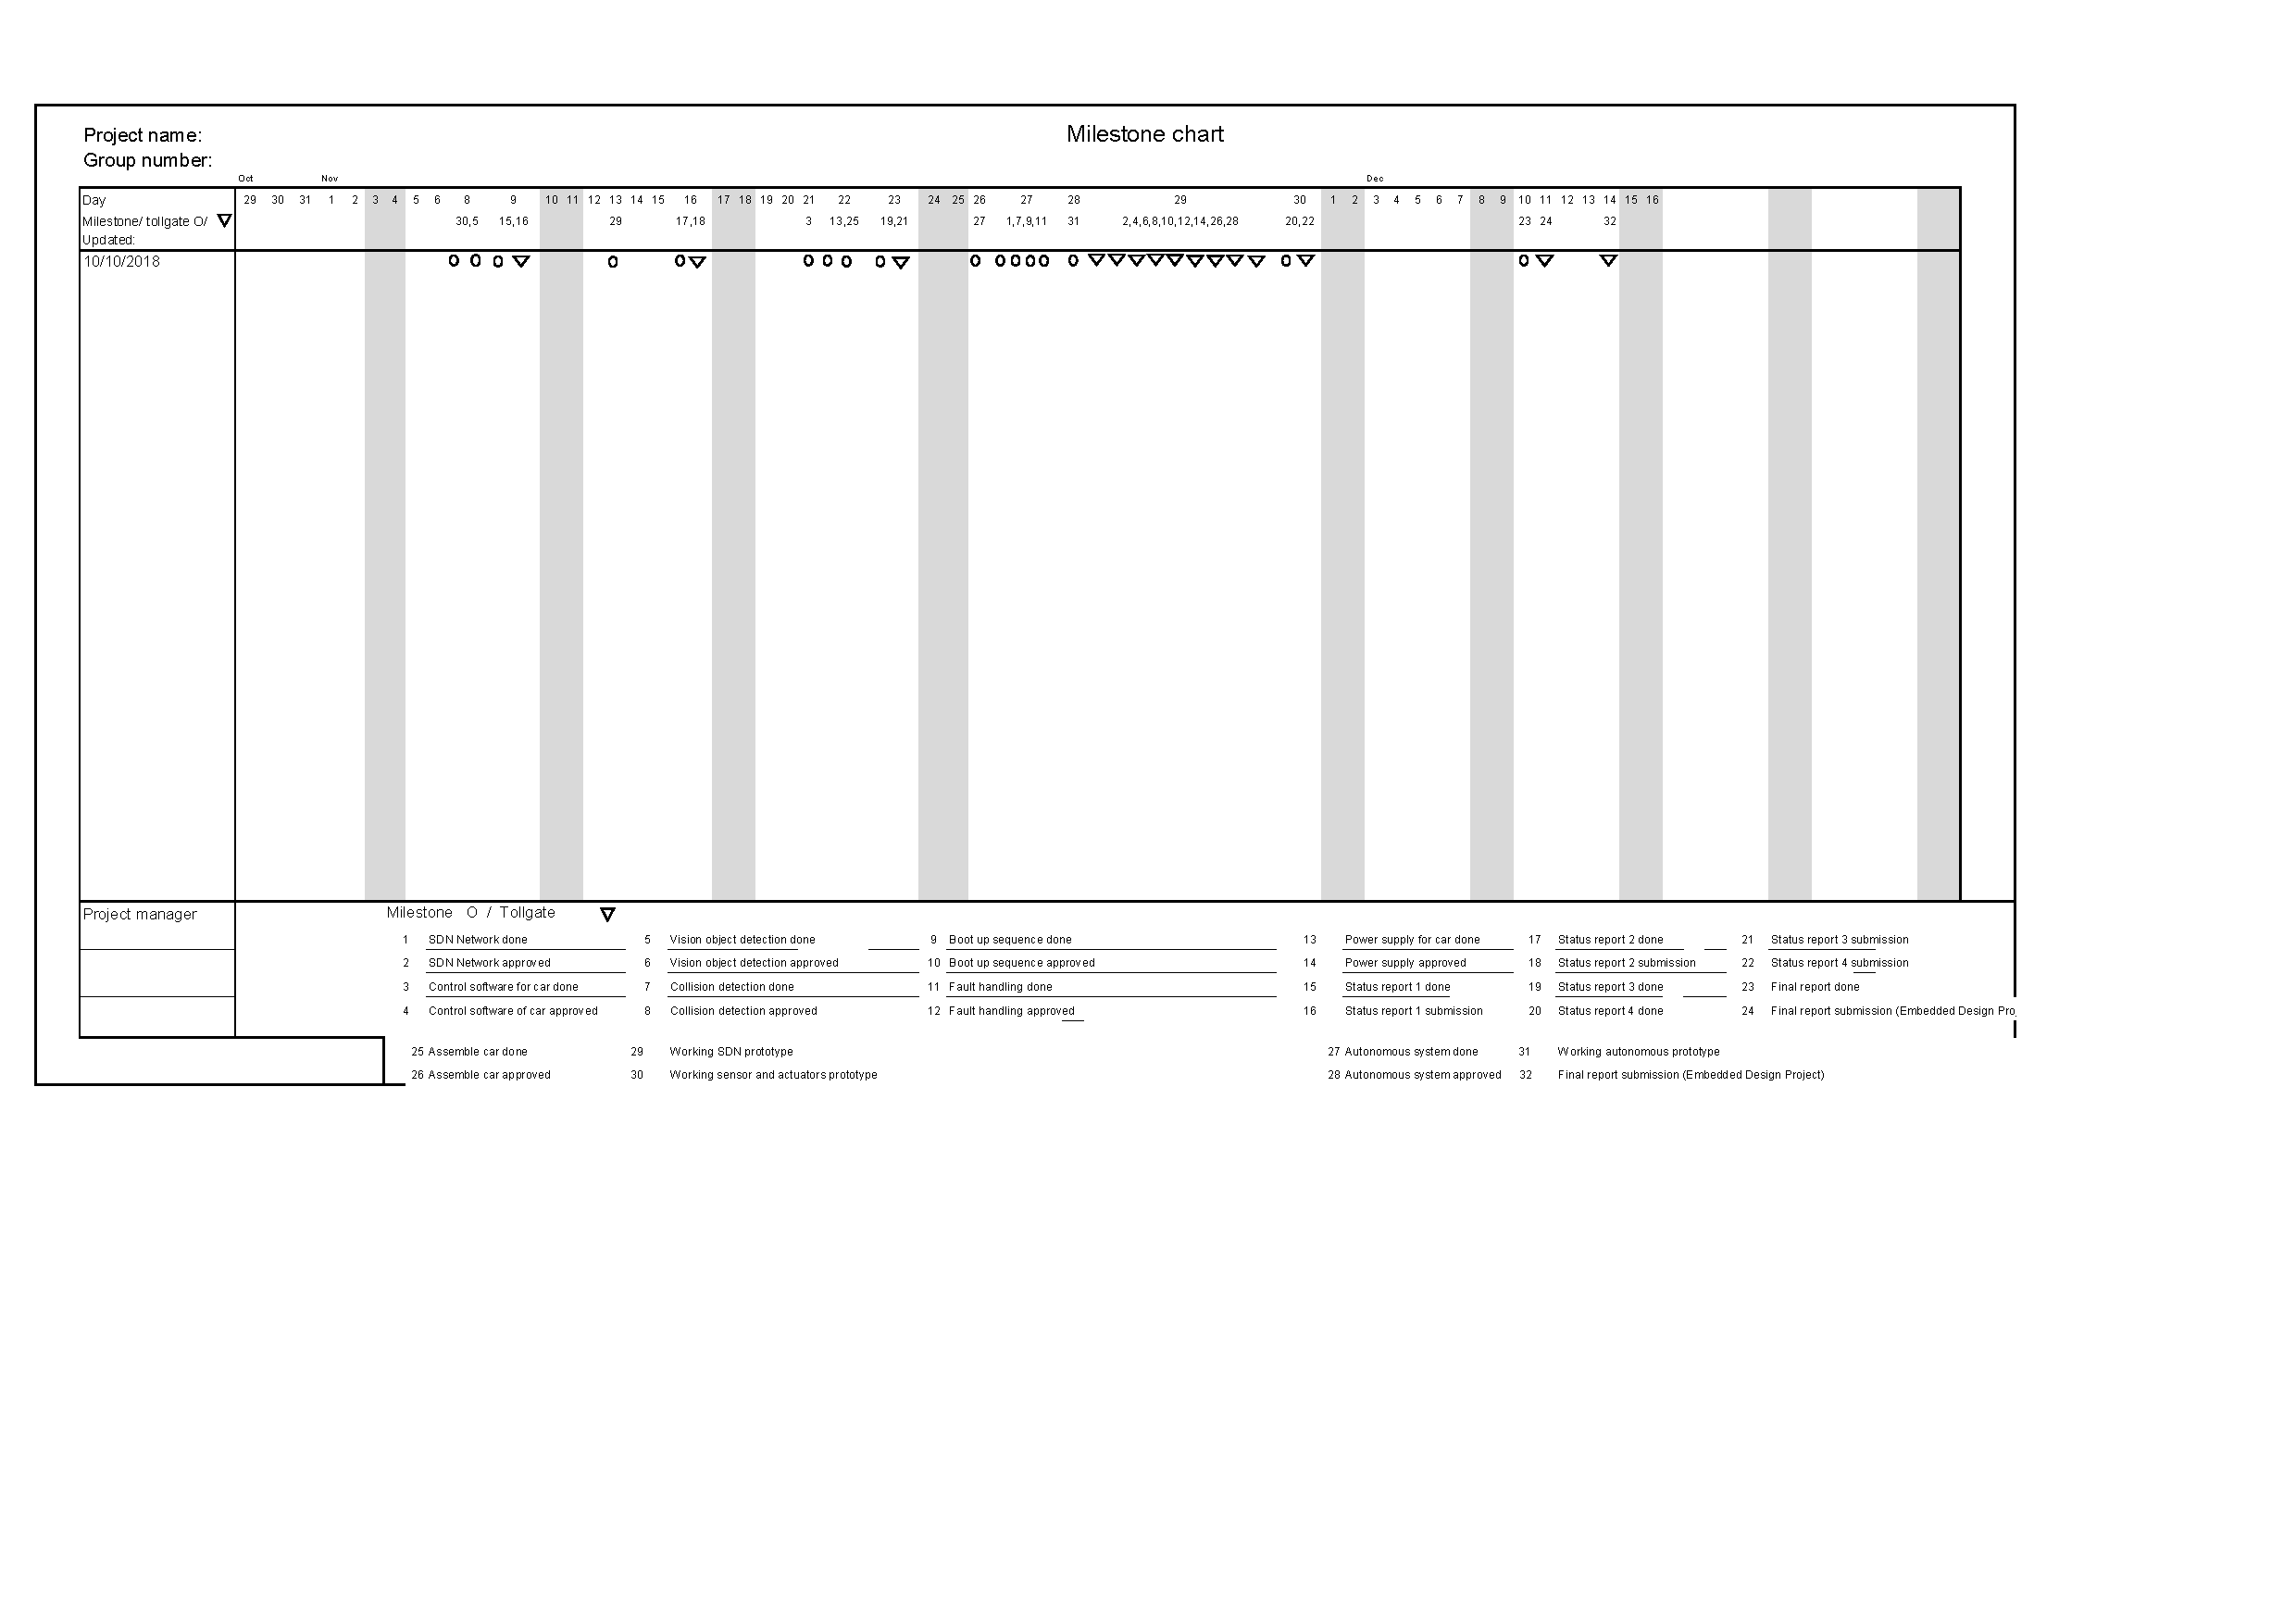
\includegraphics[width=\textwidth]{timeplan.pdf}
    \caption{The timeplan for the project.}
    \label{fig:timeplan}
\end{sidewaysfigure}
\clearpage

\section{Resource Plan}
\begin{sidewaysfigure}
    \centering
    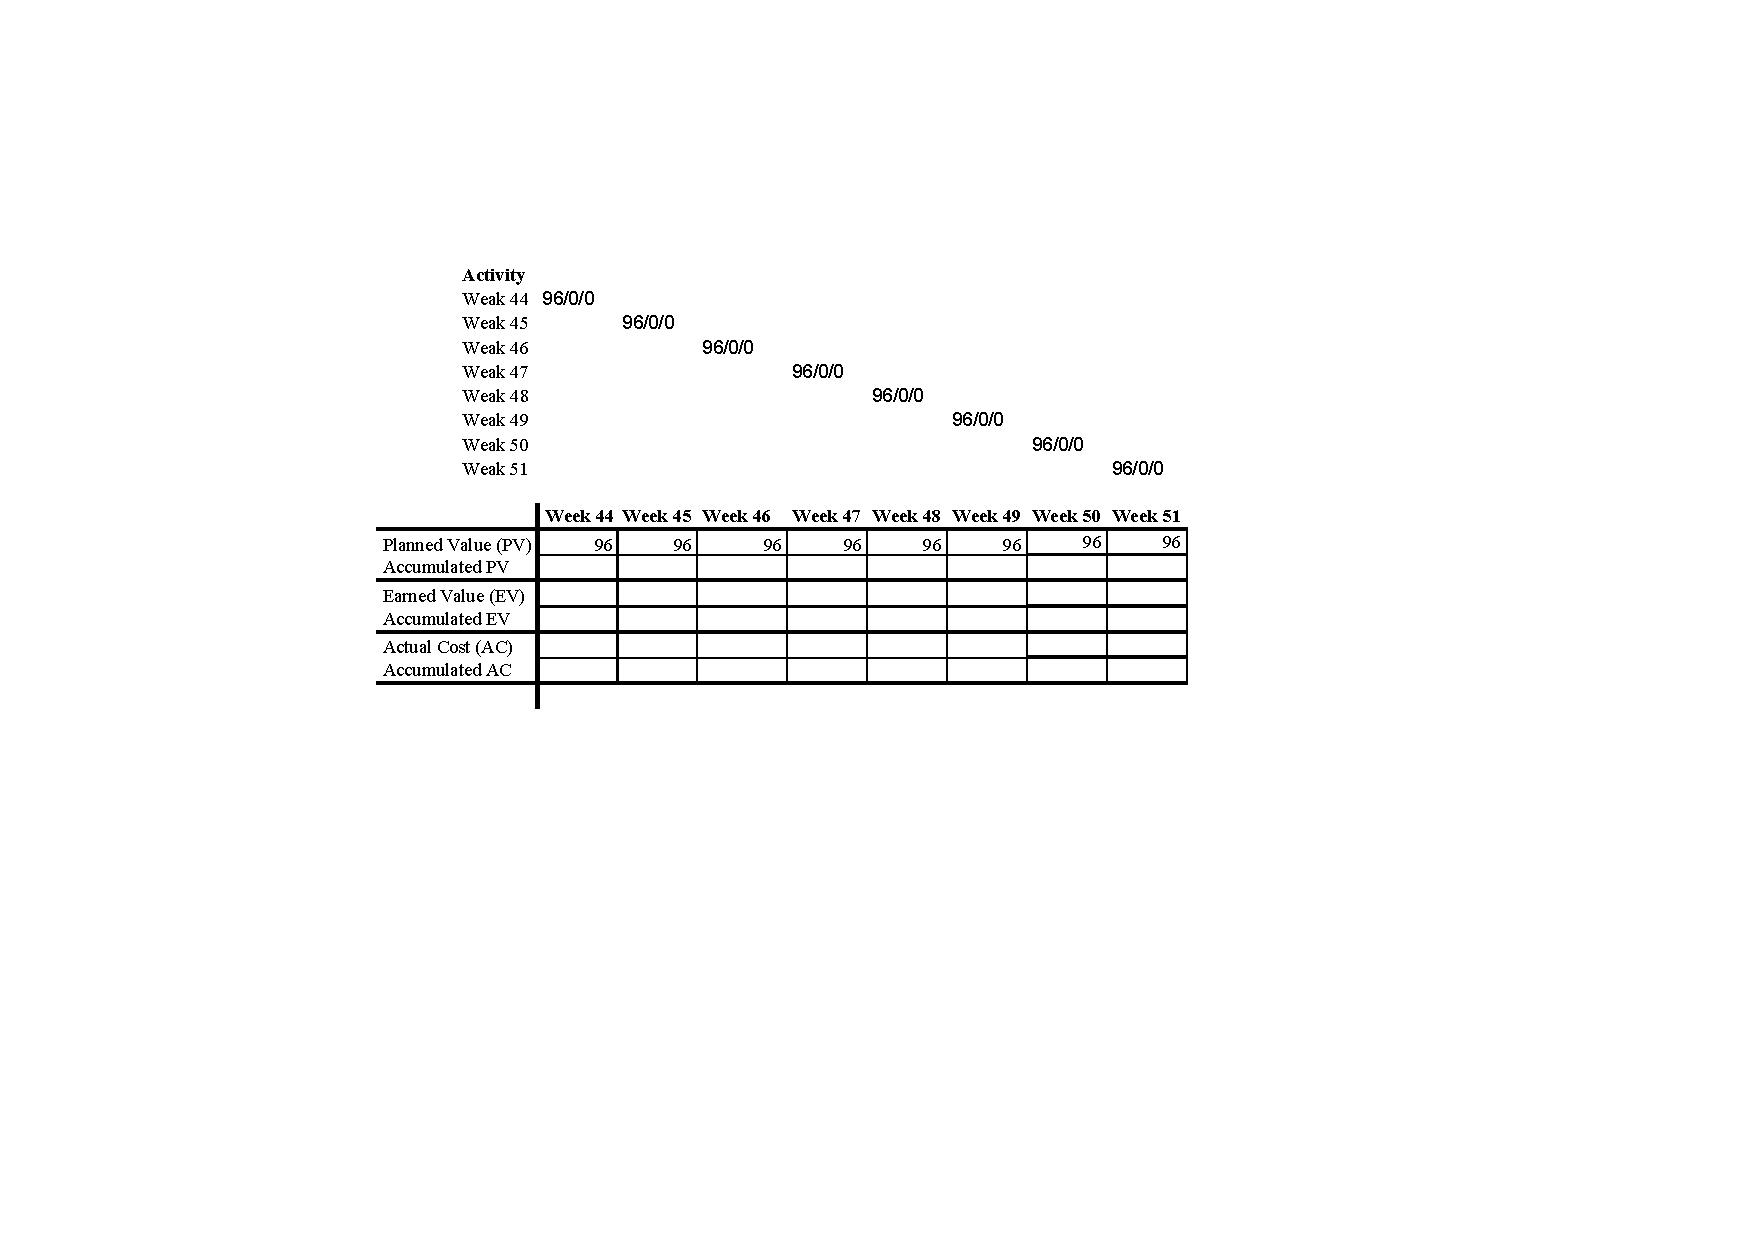
\includegraphics[scale=0.8]{evm.pdf}
    \caption{The EVM resource plan for the project.}
    \label{fig:evm}
\end{sidewaysfigure}
\clearpage

\section{Work Breakdown Structure}
The WBS was done digitally on Google Drive. It was later summarized into
Figure \ref{fig:wbs}.
\begin{sidewaysfigure}
    \centering
    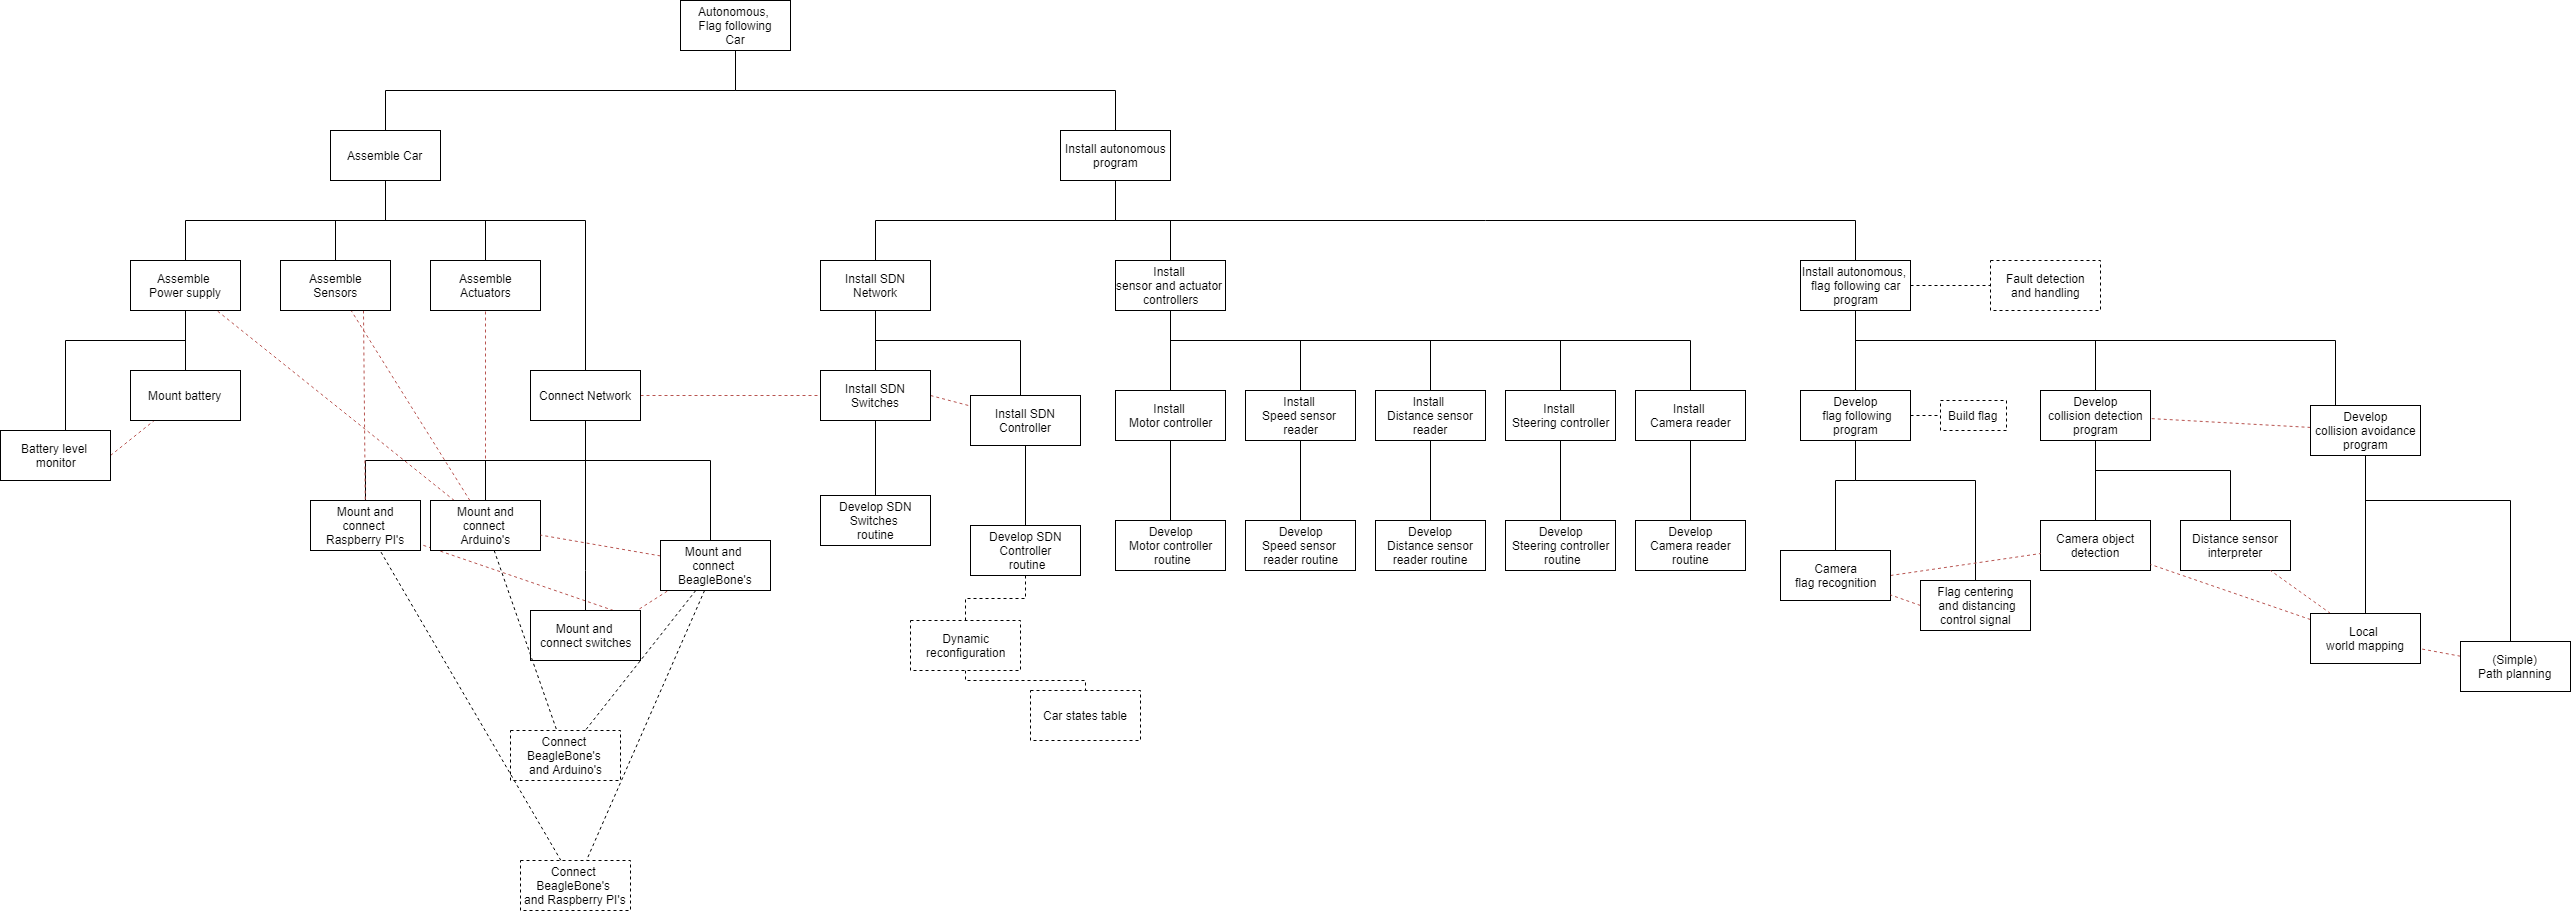
\includegraphics[width=\textwidth]{wbs.png}
    \caption{The Work Breakdown Structure for the autonomous car.}
    \label{fig:wbs}
\end{sidewaysfigure}

\end{document}
